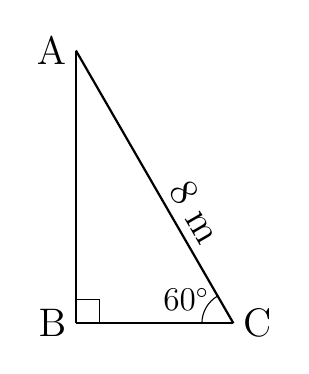
\begin{tikzpicture}[scale=1]

    % --- Coordinates (Smaller size) ---
    % Vertex B is the right-angle corner at the origin (0,0)
    \coordinate (B) at (0,0);
    % Vertex C is placed horizontally (Base reduced to 2 units for a smaller size)
    \coordinate (C) at (2,0);
    % Vertex A is calculated to maintain the 60 degree angle at C
    % height = base * tan(60) = 2 * 1.732 = 3.464
    \coordinate (A) at (0,3.464);

    % --- Triangle Sides ---
    % Drawing the segments AB, BC, and hypotenuse AC
    \draw[thick] (B) -- (A);
    \draw[thick] (B) -- (C);
    \draw[thick] (A) -- (C);

    % --- Right Angle Symbol ---
    % Square marker at vertex B
    \draw (0,0.3) -- (0.3,0.3) -- (0.3,0);

    % --- Angle Marker at C ---
    % Arc at vertex C representing the 60 degree angle
    % Arc starts at 1.6 (2.0 - 0.4)
    \draw (1.6,0) arc (180:120:0.4);
    \node[font=\large] at (1.4, 0.3) {$60^{\circ}$};

    % --- Hypotenuse Label ---
    % Measurement label changed to "8 m" as requested
    % Positioned at the midpoint of the smaller hypotenuse
    \node[above right, rotate=-60, font=\Large] at (1, 1.732) {8 m};

    % --- Point Labels (Bigger Letters) ---
    % Using font=\Large to make the vertex letters bigger
    \node[left, font=\Large] at (A) {A};
    \node[left, font=\Large] at (B) {B};
    \node[right, font=\Large] at (C) {C};

\end{tikzpicture}